%****************************************************
%	CHAPTER 3 - THEORETICAL DEVELOPMENT
%****************************************************
\chapter{Introduction to LiDAR \& Point Cloud Processing}
\label{ch:theory}

%====================================================
\section{LiDAR Characteristics and Sensors}
\label{sec:ch3:section1}
%----------------------------------------------------

\ac{LiDAR} is one of the youngest remote sensing methods, and in recent years the technology has matured greatly, increasing accessibility and allowing for its use in a wider range of applications. \ac{LiDAR} offers several advantages over traditional remote sensing methods. As an active sensing system, it does not depend on external illumination, unlike visual methods such as telephoto or stereoscopic cameras, see Figure \ref{fig:methods} for a graphical comparison of cameras, \ac{LiDAR} and \ac{Radar}. \ac{LiDAR} is also more robust to issues like poor focus, lens flare and overexposure that commonly affect optical cameras. This is due to \ac{LiDAR} sensors lacking components such as lenses and imaging sensors, which produce these effects, that optical cameras require. Additionally, certain \ac{LiDAR} sensors can penetrate vegetation, enabling ground surface mapping beneath plant cover (\cite{wangChallengesOpportunitiesLidar2021}).

Compared to \ac{Radar}, \ac{LiDAR} typically has superior mapping precision and target resolution, allowing more accurate reproductions of the target and the surrounding environment. \ac{LiDAR} makes use of electromagnetic radiation with shorter wavelengths than those typically used in \ac{Radar}, allowing for finer detail to be resolved in the collected \ac{LiDAR} data. \ac{Radar} data also often requires more complex processing and skilled individuals to extract useful information, whereas \ac{LiDAR} data is usually more straightforward to interpret (\cite{agrawalComparativeAssesmentRemote2019}).

Using \ac{LiDAR} is not without its disadvantages. \ac{LiDAR} sensors are often more expensive than other traditional remote sensing hardware and as it is a less well established method there are fewer hardware options available. Unlike cameras, which can recover non-geometric details such as target colour and texture, \ac{LiDAR} is only able to recover the three-dimensional geometry of the target. \ac{Radar} outperforms \ac{LiDAR} in various applications. It is capable of much larger detection ranges than \ac{LiDAR} and is also unaffected by adverse environmental conditions such as smoke, rain, and fog, due to its use of longer wavelength electromagnetic radiation being capable of penetrating these conditions.

%----------------------------------------------------
\begin{figure}[H]
    \centering
    \begin{minipage}{0.28\textwidth}
        \centering
        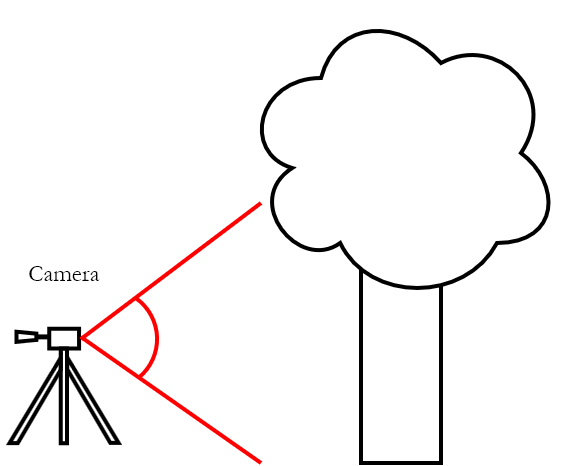
\includegraphics[width=1\linewidth]{figs/ch3/camera.png} % first figure itself
    \end{minipage}\hfill
    \begin{minipage}{0.28\textwidth}
        \centering
        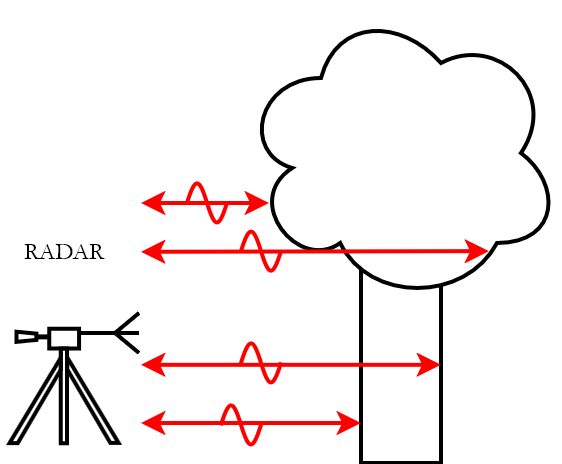
\includegraphics[width=1\linewidth]{figs/ch3/radar.png} % second figure itself
    \end{minipage}
    \begin{minipage}{0.28\textwidth}
        \centering
        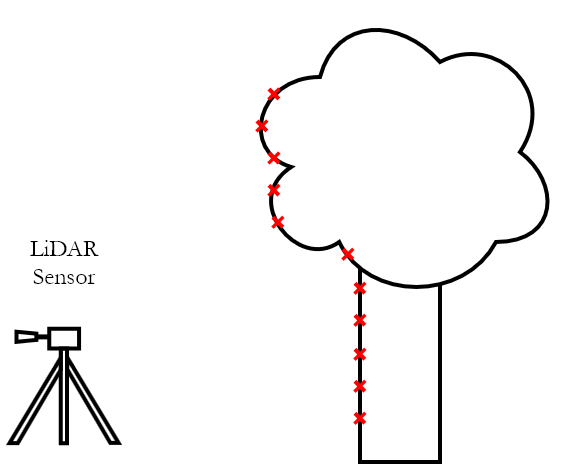
\includegraphics[width=1\linewidth]{figs/ch3/lidar.png} % first figure itself
    \end{minipage}\hfill
    \caption{\textbf{Remote Sensing Methods Comparison.}}{Cameras capture visible light and no depth information, radar uses radio waves to detect objects and measure their distance, and LiDAR uses lasers to create detailed 3D models.}
    \label{fig:methods}
\end{figure}
%----------------------------------------------------

All \ac{LiDAR} sensors suffer from beam divergence due to their use of lasers as the sensor emitter. Beam divergence is a measure of the angle at which photons diverge from the axis of the emitter over distance as the beam exits the laser aperture (\cite{jelinkovaLaserCharacteristics2013}). The steering mechanism within \ac{LiDAR} sensors may also impact the total beam divergence of the system. Beam divergence results in the laser beam or pulse exiting the sensor not as a single stream of photons, but rather as a cone of photons as shown in Figure \ref{fig:divergence}. When the beam reaches a target, the footprint of the beam will be in the shape of an ellipse with a size different to that of the beam at the aperture (\cite{kukkoMobileLaserScanning2013}). Beam divergence leads to uncertainties and errors in the reported locations of targets and their associated points in the final point cloud.

%----------------------------------------------------
\begin{figure}[H]
    \centering
    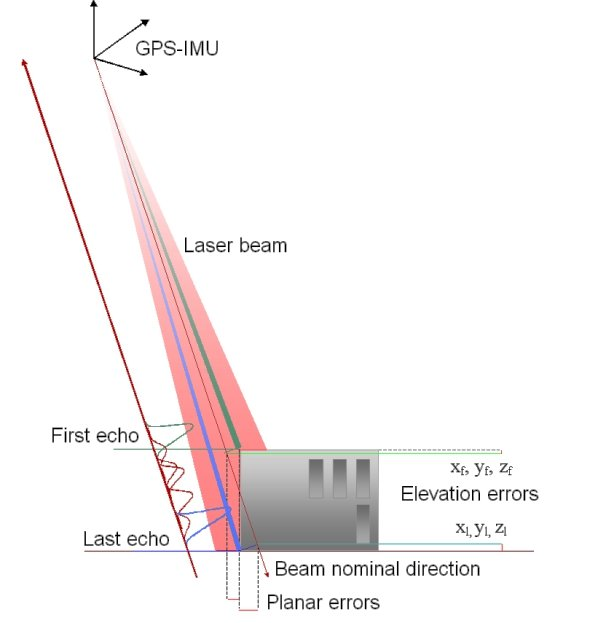
\includegraphics[width=0.45\textwidth]{figs/ch3/Beam-divergence.jpg}
    \caption{\textbf{Beam Divergence.}}{LiDAR beam divergence occurs when the emitted laser beam spreads out as it travels away from the sensor, resulting in uncertainties in the location of the target and its associated points in the final point cloud. Taken from \textcite{kukkoMobileLaserScanning2013}.}
    \label{fig:divergence}
\end{figure}
%----------------------------------------------------

Like any observation method that relies on line of sight, \ac{LiDAR} is susceptible to occlusion. If an object is blocking the line of sight between the sensor and the target, no data will be collected for that target. Self-shadowing is a phenomenon that occurs when parts of a target occlude other parts of the same target from the sensor's line of sight, see Figure \ref{fig:shadow}. This is common when the target under observation has a complex surface geometry with many protrusions and recesses or when the sensor is positioned at an oblique angle to the target. A combination of both complex target geometry and oblique sensor positioning can lead to significant portions of the target being unobserved, leading to incomplete point cloud data (\cite{landyNumericalExperimentalEvaluation2015}).

%----------------------------------------------------
\begin{figure}[H]
    \centering
    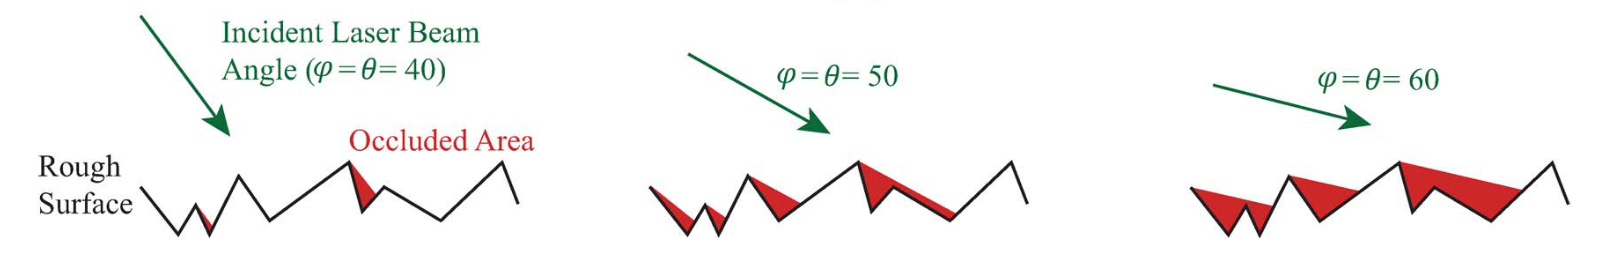
\includegraphics[width=\textwidth]{figs/ch3/shadowing.png}
    \caption{\textbf{Self-shadowing.}}{The geometry of the target and the position of the sensor can lead to parts of the target occluding itself from the sensor's line of sight, resulting in incomplete point cloud data and lost details of the target's geometry. Taken from \textcite{landyNumericalExperimentalEvaluation2015}.}
    \label{fig:shadow}
\end{figure}
%----------------------------------------------------

\ac{LiDAR} is frequently used in combination with other remote sensing methods to mitigate the disadvantages of each method and provide higher quality data. For example, \ac{LiDAR} point clouds are often complemented with optical sensor data to provide colour and texture information to the geometry data, allowing for a more wholistic representation of the target scene (\cite{wangEvolutionLiDARIts2020}).

%----------------------------------------------------
\subsection{LiDAR Sensors}
\label{subsec:ch3.section1.subsec1}

A basic \ac{LiDAR} sensor consists of four main components, a laser source, a steering mechanism to direct the laser beam, a method of detecting the returning laser pulse and a controller or processor to manage the sensor's operation and process the collected data. Various different configurations of these components exist, leading to a wide variety of \ac{LiDAR} sensor types designed for different applications (\cite{rajSurveyLiDARScanning2020}). 

Most commercial \ac{LiDAR} sensors make use of near-infrared lasers (approximately 800 to 2 500 nm) as this wavelength range is classified as eye-safe and many lasers in this range are available commercially (\cite{molebnyLaserRadarHistorical2016}). It is not uncommon for \ac{LiDAR} sensors to make use of many transceivers (laser source and detector pairs) to increase their point output rate and improve their spatial resolution. To create a 3D point cloud, a \ac{LiDAR} sensor must be capable of steering the laser beam to cover the target area. The steering mechanism used determines the \ac{FOV}, angular resolution and may impact the measurement accuracy of the sensor. Early and low-cost sensors frequently make use of optical components such as actuated mirrors or prisms to direct the laser beam across the target area. More advanced sensors make use of solid-state components such as \ac{MEMS} mirrors or phased arrays (using beam steering) to direct the laser beam without any moving parts. \ac{LiDAR} sensors that contain multiple fixed transceivers often make use of rotating platforms to achieve 360-degree coverage (\cite{rajSurveyLiDARScanning2020}). 

The most common scanning pattern created by a \ac{LiDAR} sensor is a rectangular grid pattern (N x M grid of points). Sensors that make use of rotating platforms often create circular or cylindrical scanning patterns with a set vertical resolution (usually determined by the number of transceivers) and 360-degree azimuth coverage. A less common scanning pattern is a non-repetitive rosette or flower-shaped pattern, which covers areas not scanned in previous frames. This scanning method results in a non-uniform distribution of points across its \ac{FOV}, with a high density of points in the centre of the \ac{FOV} and the number of points reducing outwards to the edges of the sensor's \ac{FOV}. To create this scanning pattern, a Risley prism (see Figure \ref{fig:risley} below) is commonly used as the steering mechanism. A Risley prism consists of two sequential wedge-shaped prisms that rotate independently to steer the laser beam. By varying the speed of rotation and direction of each prism, various scanning patterns can be created (\cite{brazealRigorousObservationModel2021}).

%----------------------------------------------------
\begin{figure}[H]
    \centering
    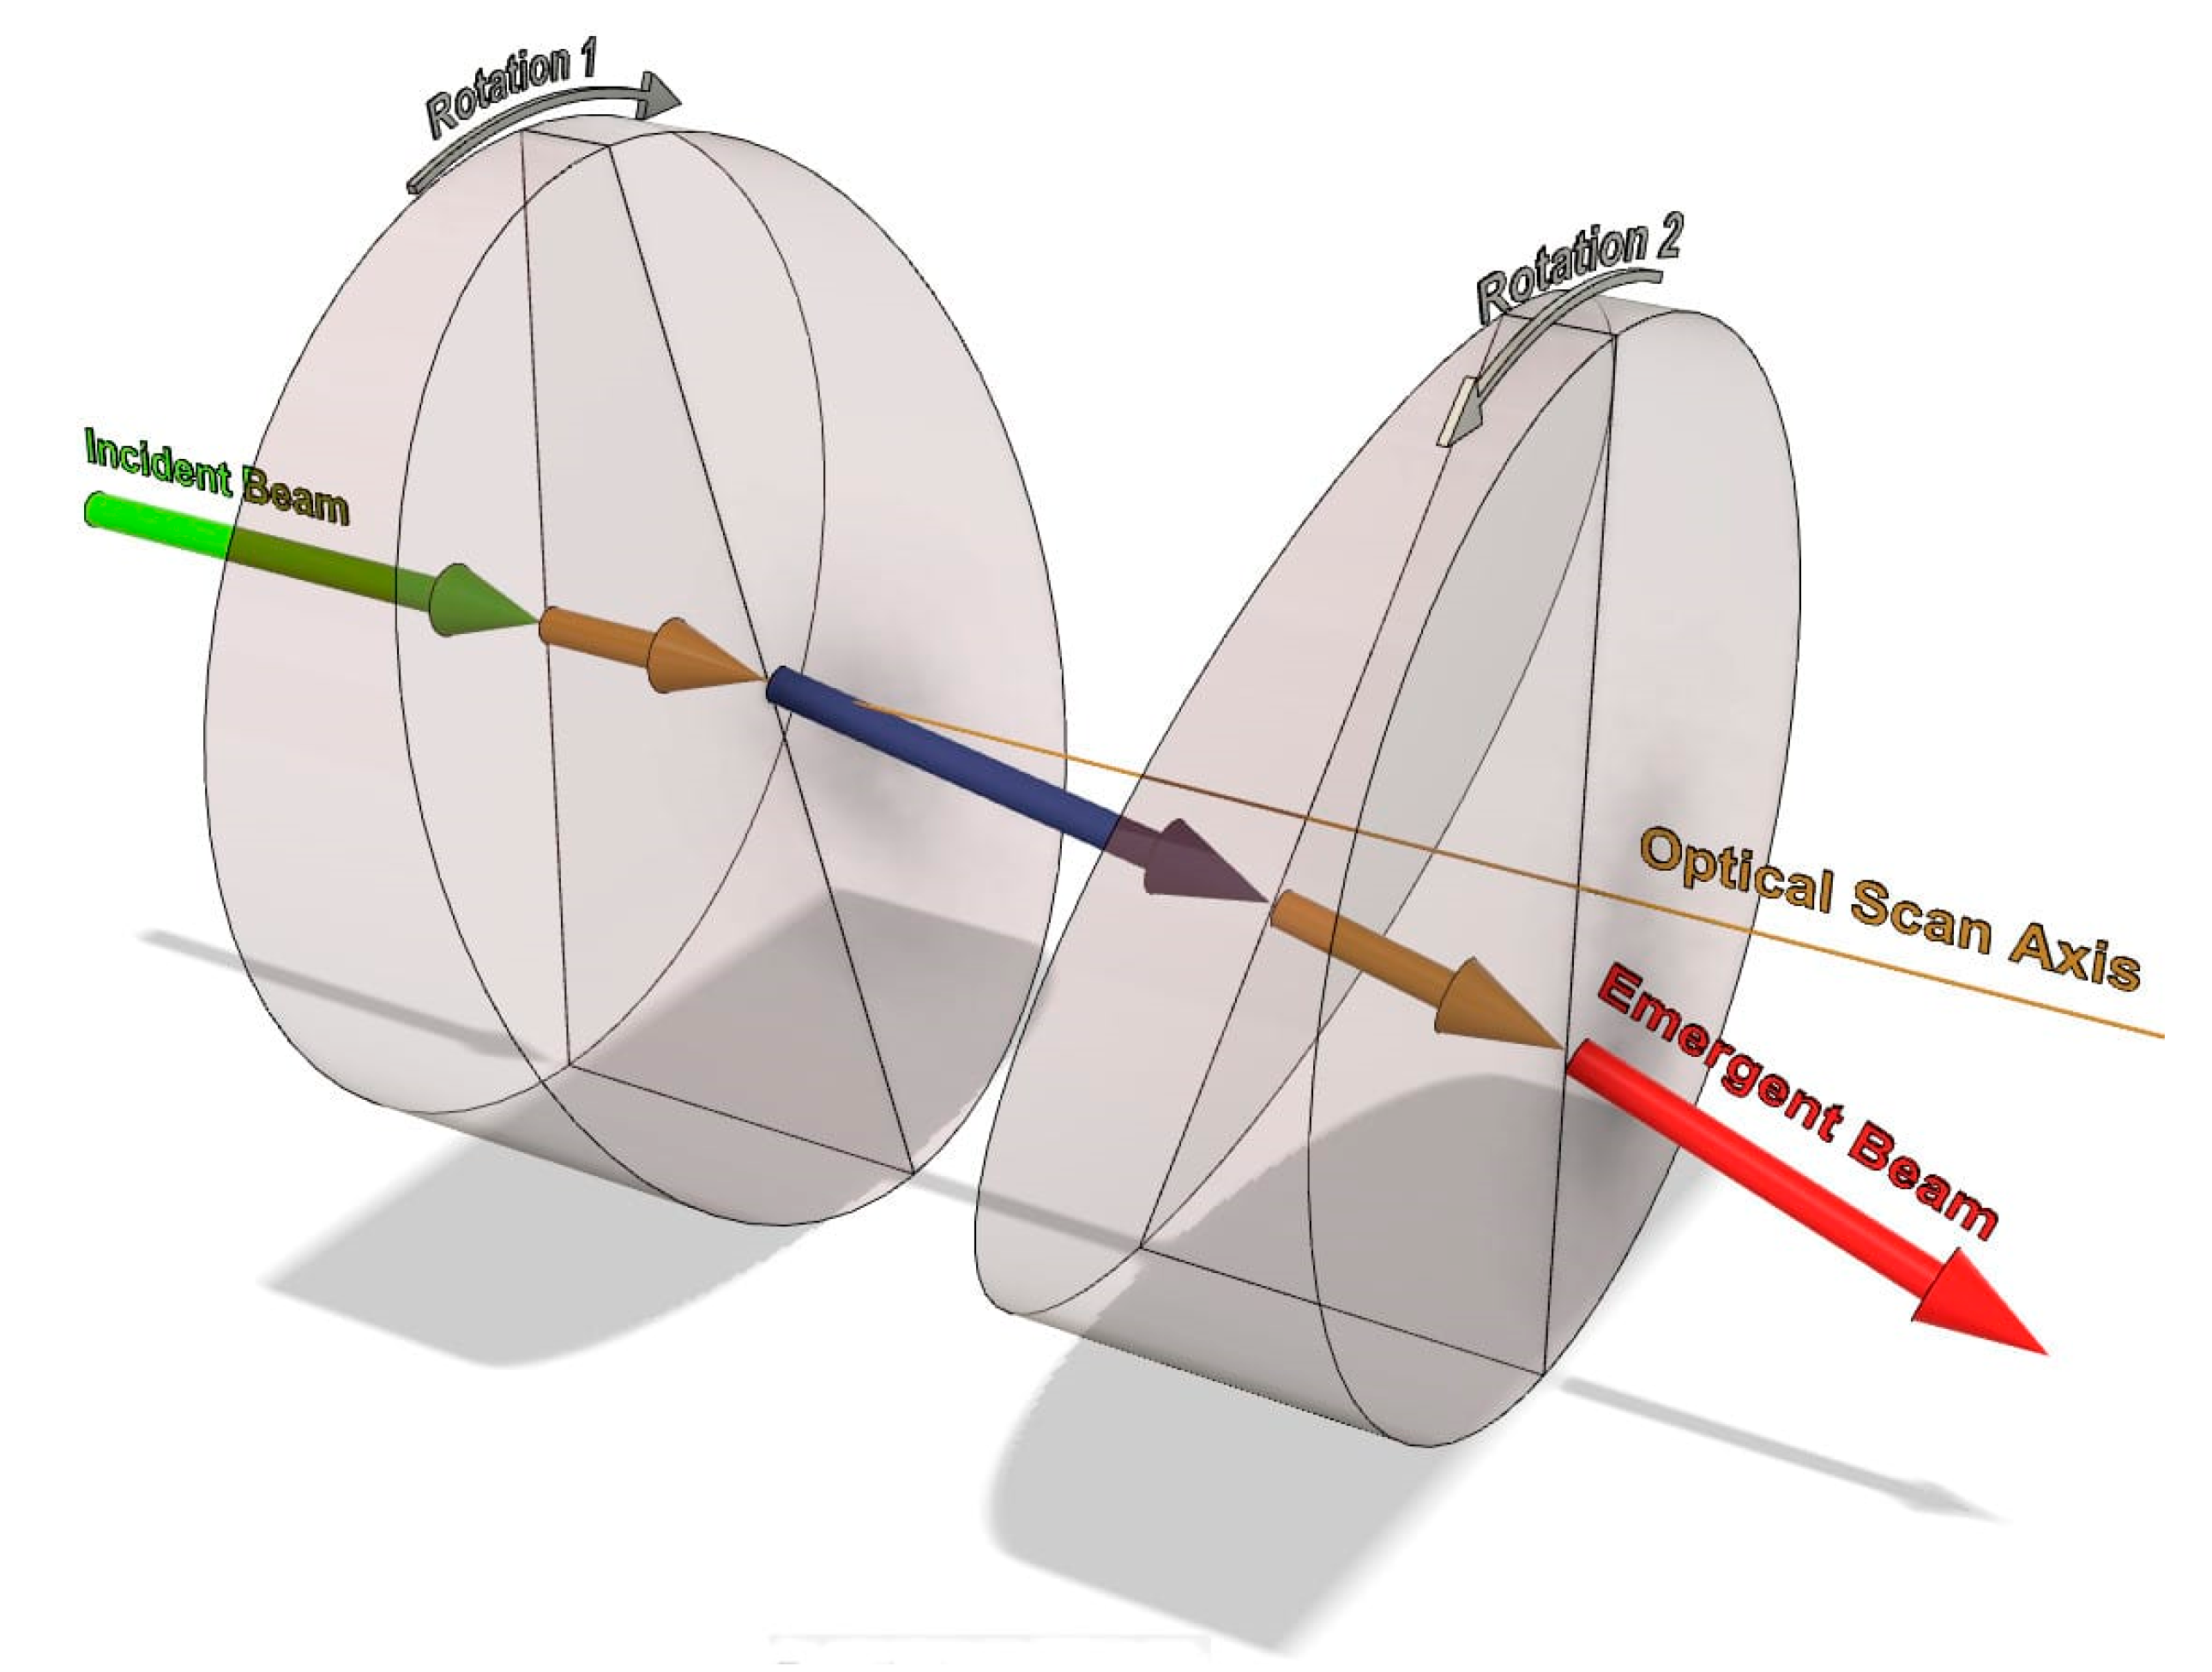
\includegraphics[width=0.5\textwidth]{figs/ch3/risley.png}
    \caption{\textbf{Risley Prism.}}{The Livox Avia makes use of a Risley prism as its steering mechanism to create its distinctive scanning patterns. The speed and direction of the prisms' rotation determine the scanning pattern produced. Taken from \textcite{brazealRigorousObservationModel2021}.}
    \label{fig:risley}
\end{figure}
%----------------------------------------------------

Many \ac{LiDAR} sensors are capable of detecting how much energy is returned to the sensor from each emitted laser pulse, known as the point's return intensity. The return intensity is influenced by various factors including the distance to the target, the target's reflectivity, angle of incidence and environmental conditions. This information can be useful in point cloud processing to help identify different materials or surfaces within the point cloud data (\cite{harrapOverviewLIDARCollection2010}).

Some \ac{LiDAR} sensors are capable of measuring multiple returns from a single output pulse (\cite{deemsLidarMeasurementSnow2013}). This is possible when the object hit by the laser pulse does not reflect or absorb all the output energy but allows some to pass through itself, as shown in Figure \ref{fig:multi_return}. This is common when the laser pulse hits semi-transparent objects such as vegetation or water. If this occurs multiple times for a single laser pulse, and the sensor is capable of detecting all of these returns, it is possible for a sensor to record more returned points than output laser pulses. These multiple returns can provide additional information about the target scene, such as the height of vegetation relative to the ground surface.

%----------------------------------------------------
\begin{figure}[H]
    \centering
    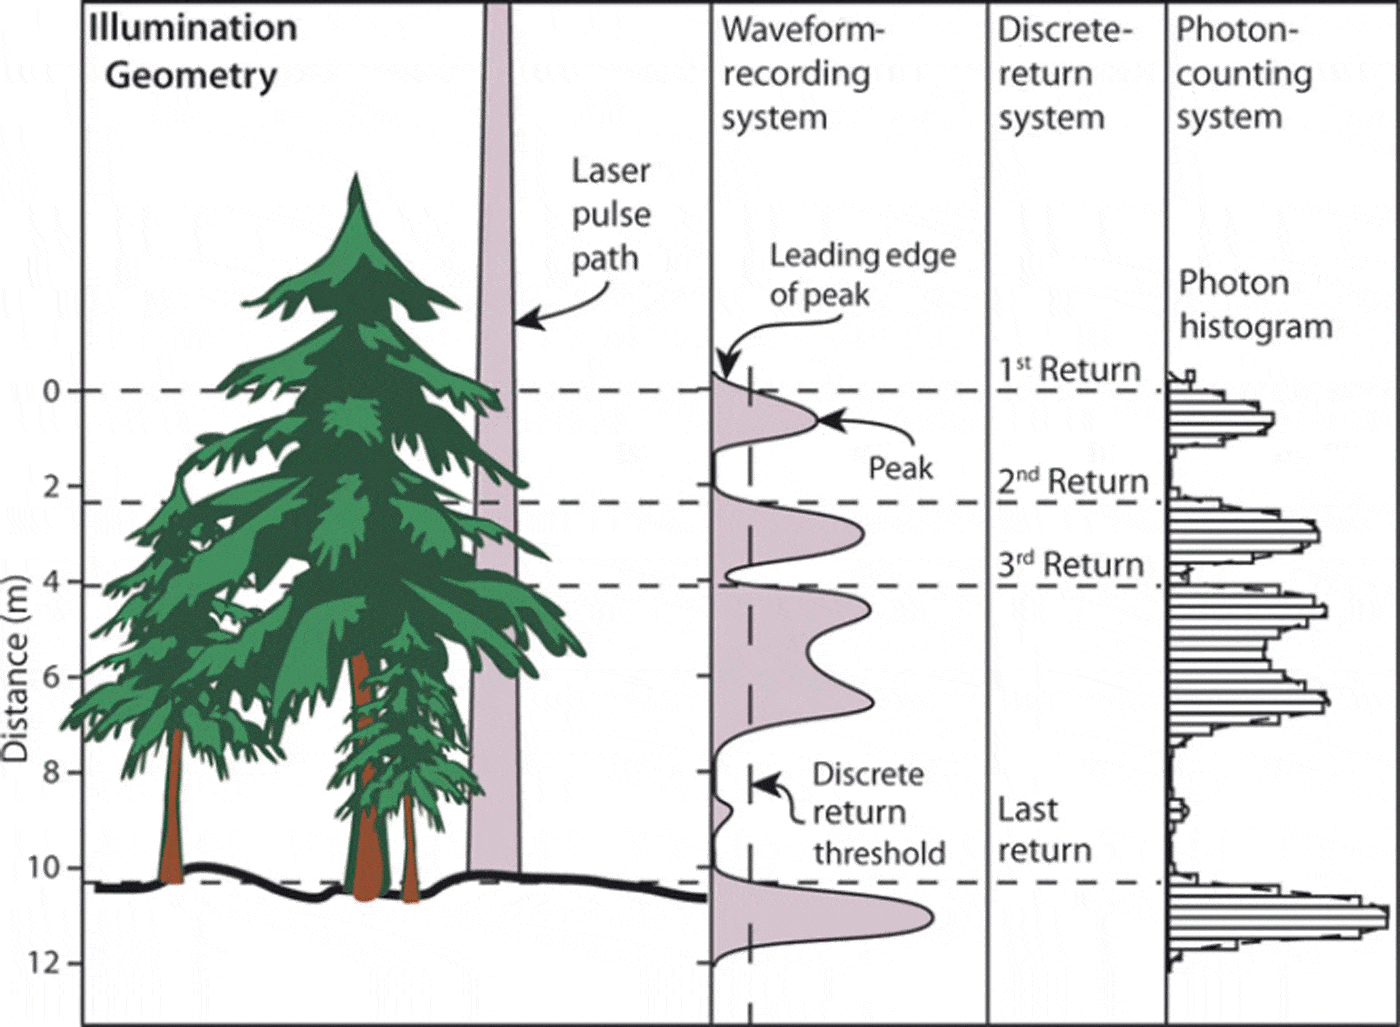
\includegraphics[width=0.42\textwidth]{figs/ch3/multi_return.png}
    \caption{\textbf{Multiple Returns from a Single Pulse.}}{A single laser pulse emitted from a sensor can produce multiple returns if the pulse hits semi-transparent objects. Taken from \textcite{lefskyLidarRemoteSensing2002}.}
    \label{fig:multi_return}
\end{figure}
%----------------------------------------------------

%====================================================
\section{Livox Avia}
\label{sec:ch3:section2}
%----------------------------------------------------

The sensor used to collect data for this investigation was the Livox Avia, see Figure \ref{fig:avia}. The Avia is a low-cost \ac{LiDAR} sensor produced by \href{https://www.livoxtech.com/}{Livox Technology}, a subsidiary of DJI. The sensor is designed for use in various typical \ac{LiDAR} applications including surveying, mapping, and autonomous systems. The Avia is a solid-state laser and Risley prism-based \ac{LiDAR} sensor with a built-in \ac{IMU}. The sensor makes use of a 905 nm near-infrared laser. 

The Avia has the ability to detect each point's return intensity. It records each point's return intensity as an 8-bit value ranging from 0 to 255, with 0 being the least returned energy and 255 being the most returned energy. The sensor has the ability to record multiple returns from a single output pulse. It can record up to three returns per pulse.

%----------------------------------------------------
\begin{figure}[H]
    \centering
    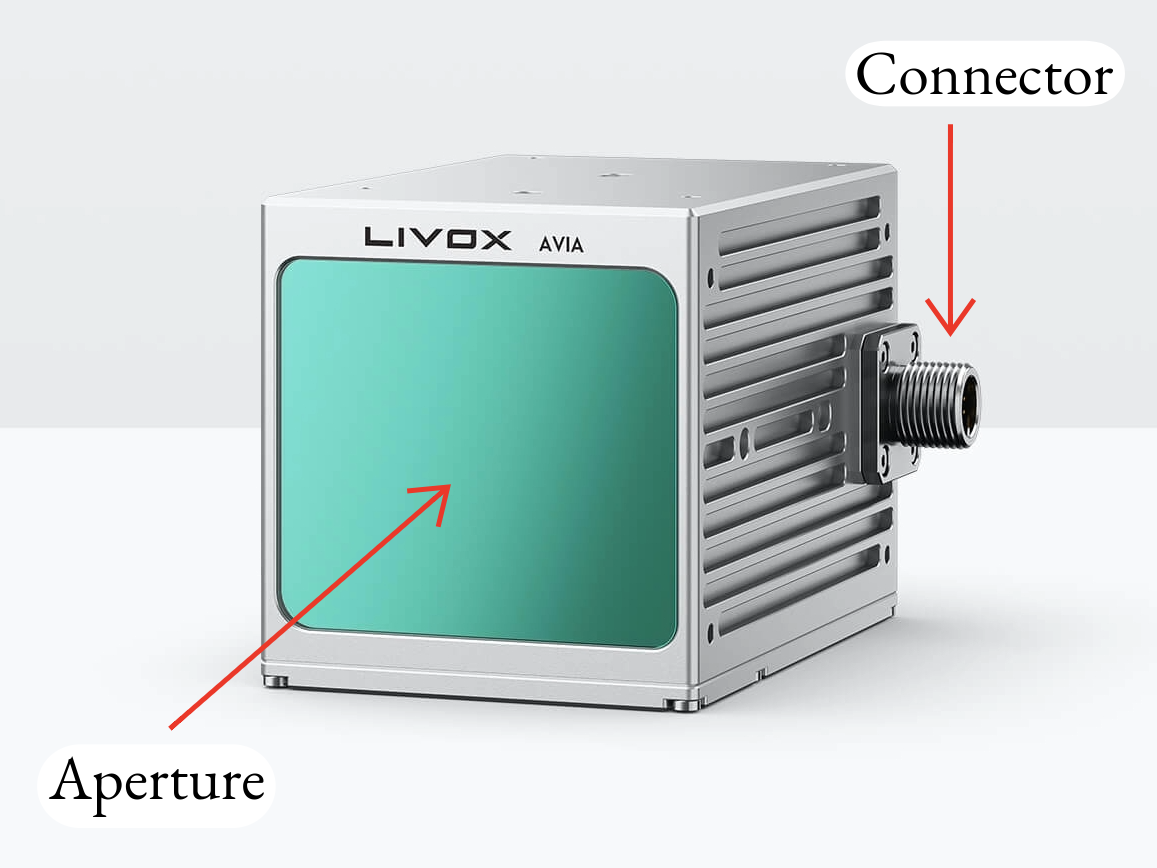
\includegraphics[width=0.42\textwidth]{figs/ch3/avia1.png}
    \caption{\textbf{Livox Avia.}}{Taken from \textcite{AviaLiDARSensor}.}
    \label{fig:avia}
\end{figure}
%----------------------------------------------------

The Livox Avia has a listed beam divergence of 0.28° x 0.03° along its vertical and horizontal planes. This results in the emitted beam, if falling on a target perfectly perpendicular to the axis of propagation at a distance of 50 meters, having the form of an ellipse with the approximate dimensions of 244.35 mm in height and 26.18 mm in width. Further specifications of the sensor are listed in Table \ref{tab:AVIA_spec} below.

The Avia has two built-in scanning patterns, a repetitive and a non-repetitive pattern. The repetitive scanning pattern scans the target area in a narrow horizontal band, providing a more uniform point density per frame when compared to the non-repetitive mode, see Figure \ref{fig:rep}. The non-repetitive scanning pattern scans the target with a rosette-shaped pattern which rotates as it scans, covering areas not scanned in previous frames, see Figure \ref{fig:non_rep}. This scanning method results in a non-uniform distribution of points across its \ac{FOV}. There is a high density of points in the centre of the \ac{FOV}, with the number of points reducing outwards to the edges of the sensor's \ac{FOV}. Each scanning pattern produces point cloud frames at a rate of 10 Hz, with each frame containing 24,000 points in single return mode. A complete frame of the repetitive scanning pattern resembles the third frame of Figure \ref{fig:rep}, while a complete frame of the non-repetitive scanning pattern resembles the second frame of Figure \ref{fig:non_rep}. 

%----------------------------------------------------
\begin{figure}[H]
    \centering
    \begin{minipage}{0.33\textwidth}
        \centering
        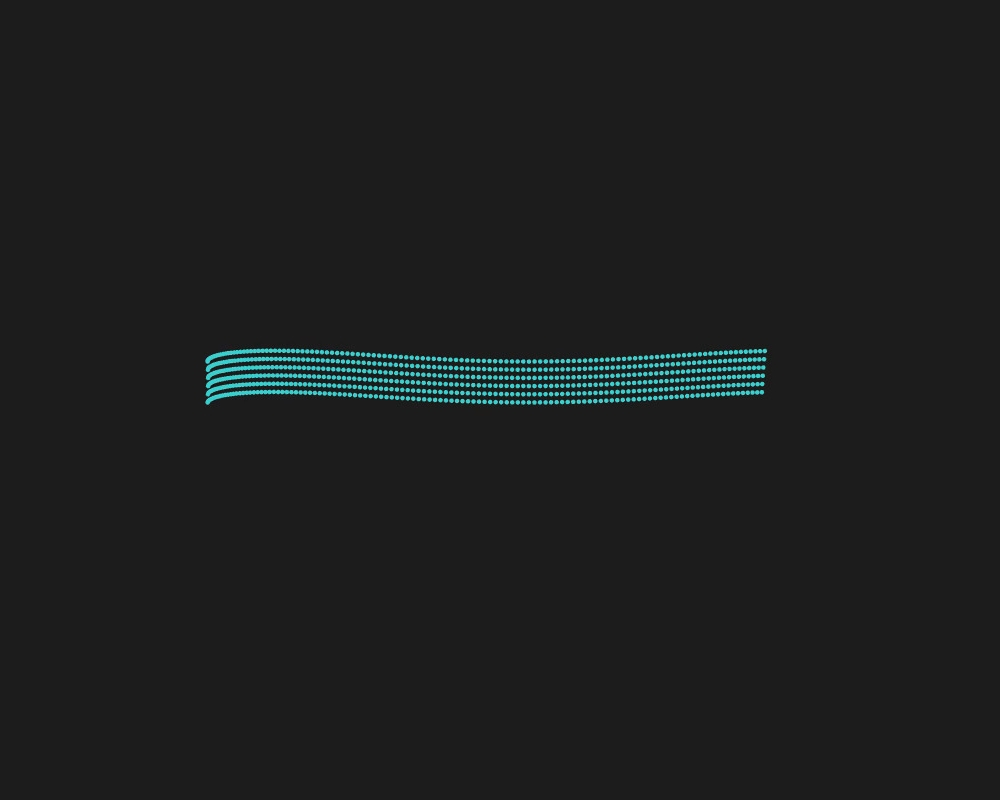
\includegraphics[width=1\linewidth]{figs/ch3/rep0.jpg} % first figure itself
    \end{minipage}\hfill
    \begin{minipage}{0.33\textwidth}
        \centering
        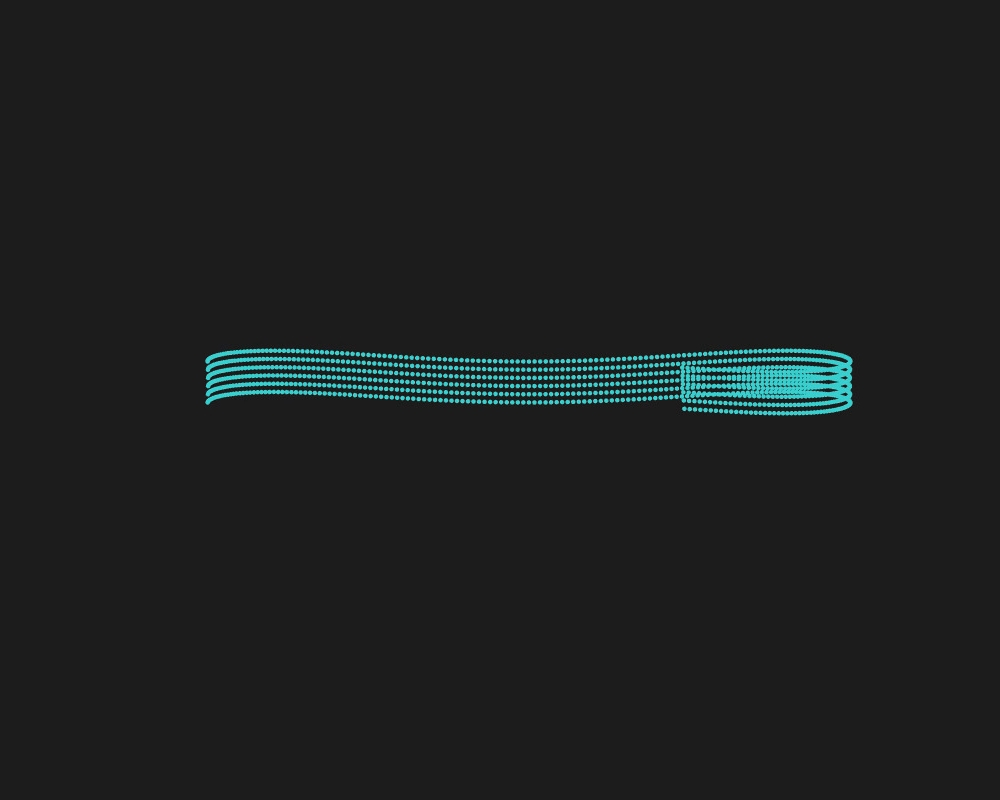
\includegraphics[width=1\linewidth]{figs/ch3/rep1.jpg} % second figure itself
    \end{minipage}
    \begin{minipage}{0.33\textwidth}
        \centering
        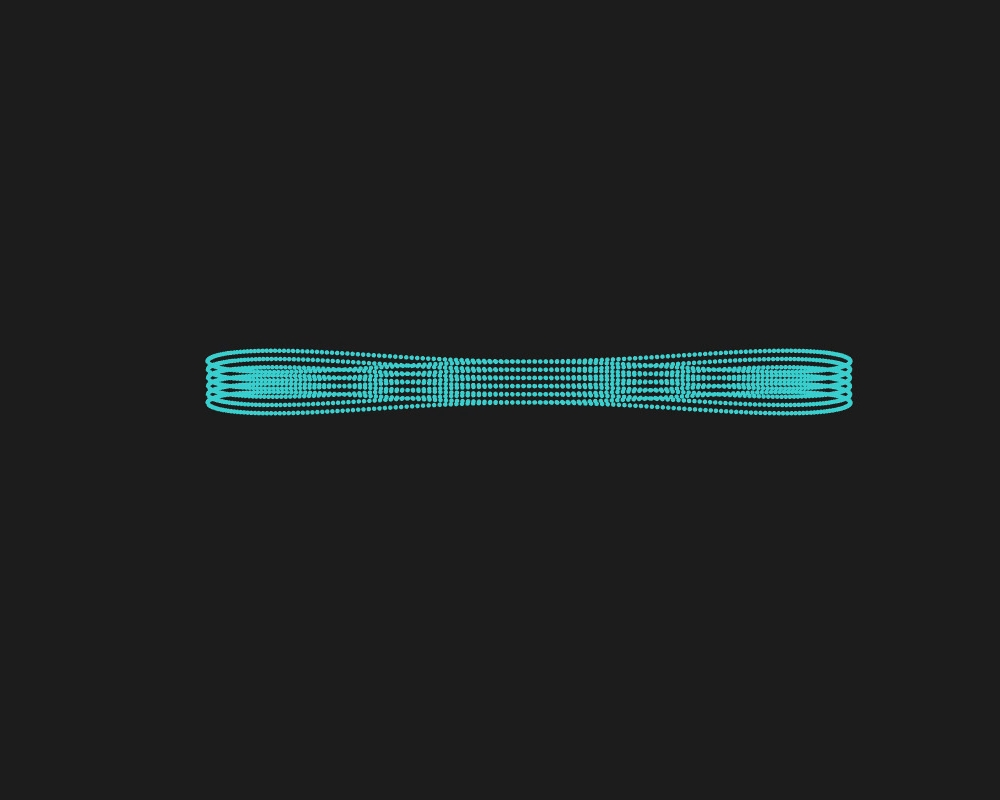
\includegraphics[width=1\linewidth]{figs/ch3/rep2.jpg} % first figure itself
    \end{minipage}\hfill
    \caption{\textbf{Livox Avia Repetitive Scanning Pattern.}}{The Avia's non-repetitive scanning pattern produces a point cloud with a roughly rectangular \ac{FOV} and consistent point density. Taken from \textcite{AviaLiDARSensor}.}
    \label{fig:rep}
\end{figure}
%----------------------------------------------------

%----------------------------------------------------
\begin{figure}[H]
    \centering
    \begin{minipage}{0.33\textwidth}
        \centering
        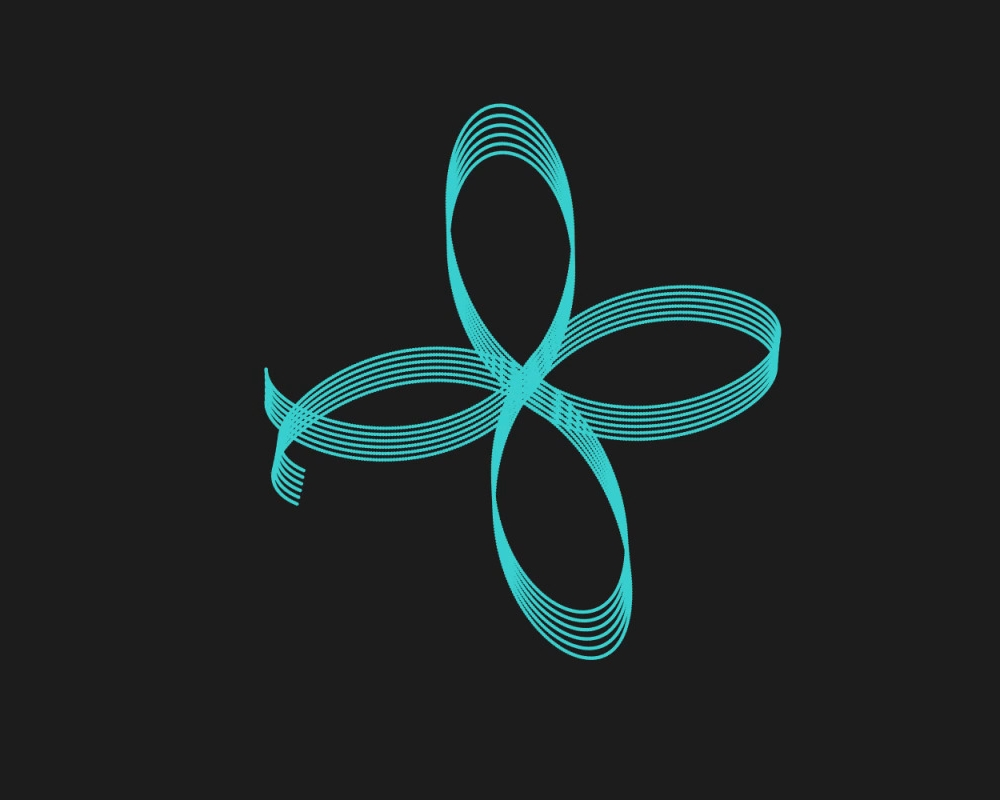
\includegraphics[width=1\linewidth]{figs/ch3/norep0.jpg} % first figure itself
    \end{minipage}\hfill
    \begin{minipage}{0.33\textwidth}
        \centering
        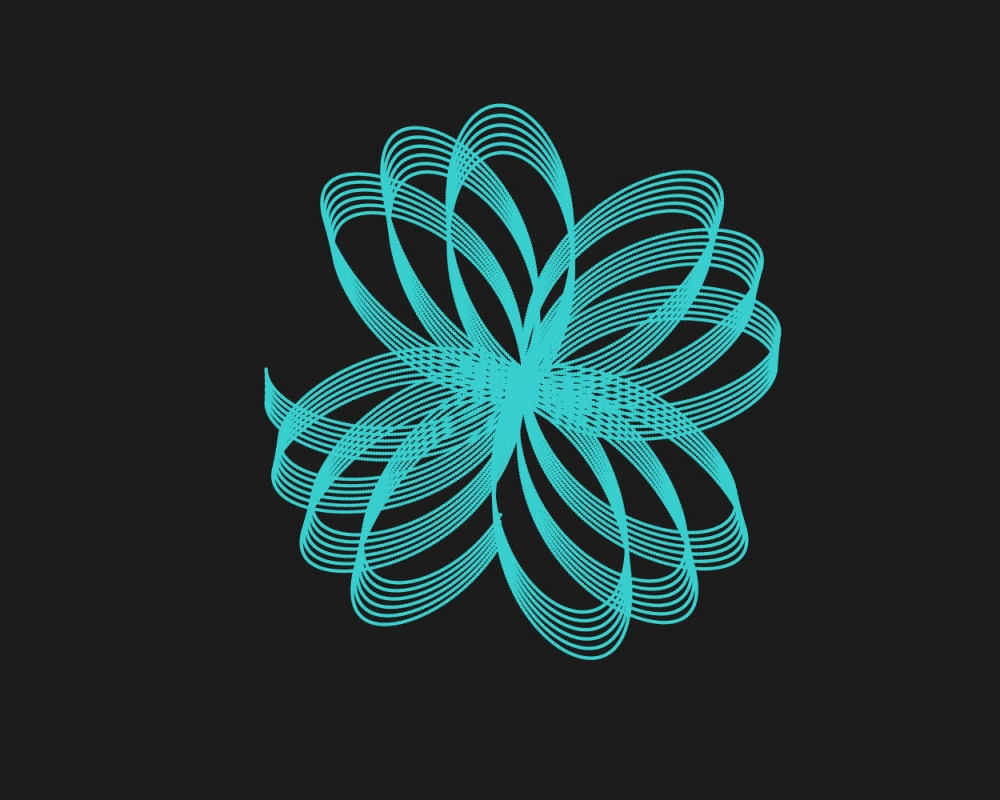
\includegraphics[width=1\linewidth]{figs/ch3/norep1.jpg} % second figure itself
    \end{minipage}
    \begin{minipage}{0.33\textwidth}
        \centering
        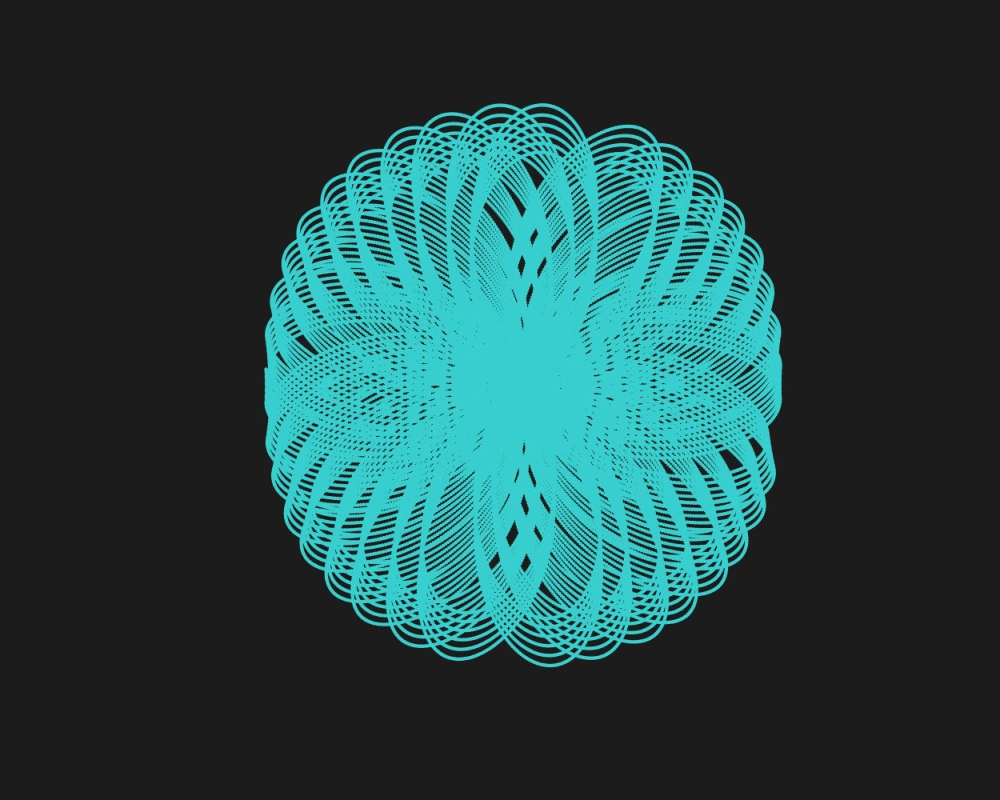
\includegraphics[width=1\linewidth]{figs/ch3/norep2.jpg} % first figure itself
    \end{minipage}\hfill
    \caption{\textbf{Livox Avia Non-Repetitive Scanning Pattern.}}{The Avia's non-repetitive scanning pattern produces a point cloud with a circular \ac{FOV} and non-uniform point density, with a high density of points in the centre of the \ac{FOV} and the number of points reducing outwards to the edges of the sensor's \ac{FOV}. Taken from \textcite{AviaLiDARSensor}.}
    \label{fig:non_rep}
\end{figure}
%----------------------------------------------------

%----------------------------------------------------
\begin{table}[H]
\centering
\caption{Livox Avia Specifications.}
\begin{tabular}{|l|l|lll}
\cline{1-2}
\textbf{Parameter}              & \textbf{Value}                        &  &  &  \\ \cline{1-2}
Laser Wavelength                & 905 nm                                &  &  &  \\ \cline{1-2}
Laser Safety                    & Class 1 (Safe for eyes)               &  &  &  \\ \cline{1-2}
Detection Range (@ 100 klx)     & \begin{tabular}[c]{@{}l@{}}190 m @ 10\% reflectivity\\ 230 m @ 20\% reflectivity\\ 320 m @ 80\% reflectivity\end{tabular} &  &  &  \\ \cline{1-2}
Detection Range (@ 0 klx)       & \begin{tabular}[c]{@{}l@{}}190 m @ 10\% reflectivity\\ 260 m @ 20\% reflectivity\\ 450 m @ 80\% reflectivity\end{tabular} &  &  &  \\ \cline{1-2}
Repetitive Pattern \ac{FOV}     & 70.4° (H) × 4.5° (V)                  &  &  &  \\ \cline{1-2}
Non-repetitive Pattern \ac{FOV} & 70.4° (H) × 77.2 (V)                  &  &  &  \\ \cline{1-2}
Distance Random Error           & 1$\sigma$ (@ 20 m) $<$ 2 cm           &  &  &  \\ \cline{1-2}
Point Rate                      & 240,000 points/s                      &  &  &  \\ \cline{1-2}
Beam Divergence                 & 0.28° (Vertical) x 0.03° (Horizontal) &  &  &  \\ \cline{1-2}
IMU                             & Bosch Sensortec BMI088                &  &  &  \\ \cline{1-2}
Operating Temperature Range     & -20° to 65° C                         &  &  &  \\ \cline{1-2}
IP Rating                       & IP67                                  &  &  &  \\ \cline{1-2}
Dimensions                      & 91 x 61.2 x 64.8 mm                   &  &  &  \\ \cline{1-2}
\end{tabular}
\label{tab:AVIA_spec}
\end{table}
%----------------------------------------------------

%====================================================
\section{Point Cloud Processing}
\label{sec:ch3:section3}
%----------------------------------------------------

Historically, \ac{LiDAR} was predominantly used in airborne applications for environmental mapping and surveying. However, with the recent advancements in \ac{LiDAR} technology, it has seen increased use in urban settings and aboard mobile and autonomous platforms (\cite{brazealRigorousObservationModel2021}). This shift has led to an increased focus on point cloud processing methods developed for urban environments and autonomous navigation, with fewer studies on improving pre-existing methods or the development of new methods for natural environments.

Many common point cloud processing methods are built around the assumption that the point cloud being worked upon is in the format of a standard (M x N) grid layout. Methods such as point cloud registration (obtaining the transformation between two point clouds (\cite{huangComprehensiveSurveyPoint2021})), clustering and model fitting often use the assumption of a constant grid with a constant number of points per frame to achieve their outputs. To bypass this limitation it is common for point clouds to be downsampled through a grid filter to achieve the desired format (\cite{3DPointCloud}).

In the Avia's repetitive scanning pattern (see Figure \ref{fig:rep}), the sensor produces a point cloud with a roughly rectangular \ac{FOV} and consistent point density, which is suitable for downsampling and grid filtering. Point clouds produced by the non-repetitive scanning pattern (see Figure \ref{fig:non_rep}) are circular and do not have uniform point density and do not have fixed locations for each point in the \ac{FOV}. These point clouds are thus not ideal for downsampling and grid filtering, as demonstrated in Figure \ref{fig:grid}.

%----------------------------------------------------
\begin{figure}[H]
    \centering
    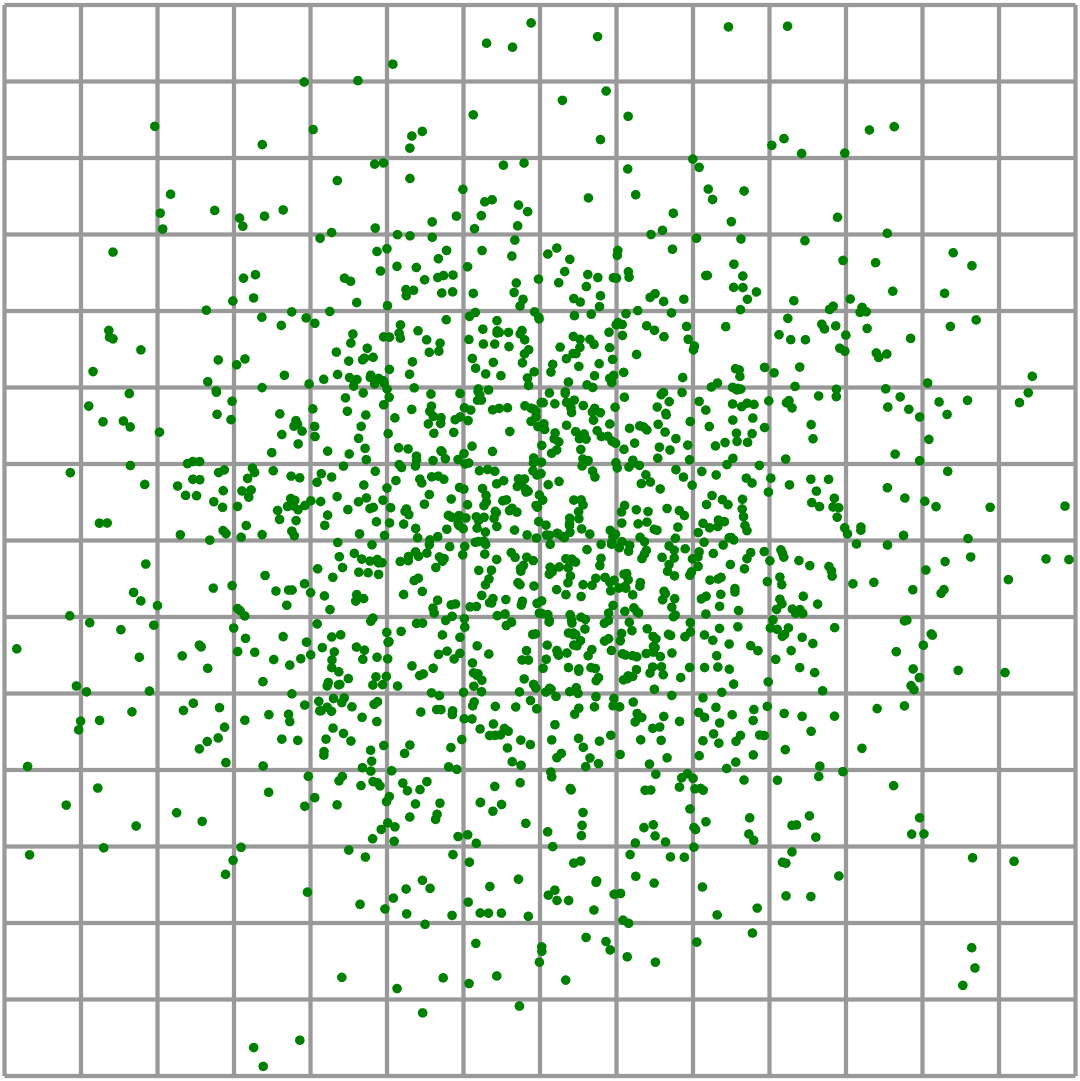
\includegraphics[width=0.5\textwidth]{figs/ch3/grid.png}
    \caption{\textbf{Irregular Density Point Cloud and Filtering Grid.}}{Visualisation of an irregular density point cloud overlaid with a filtering grid. The irregular point density makes it challenging to apply uniform filtering techniques.}
    \label{fig:grid}
\end{figure}
%----------------------------------------------------

Many processing methods are also based on the assumption that the environment data are collected from will contain predominantly objects made of simple geometries. For example, a scene in an urban environment will contain many objects consisting of planar surfaces and cuboid shapes such as roads, buildings and vehicles. The environment that data for this investigation was captured from contains none of these simple shapes, with the geometry of the pancake floes being irregular and superimposed upon complex ocean surface waves.

%----------------------------------------------------
\subsection{Plane Fitting}
\label{subsec:ch3.section3.subsec1}

Plane fitting is a common method used in point cloud processing to identify and locate planar surfaces within a point cloud. Plane fitting is commonly used to identify features such as walls, roads, and building facades in urban settings. This assists in transforming raw point cloud data into useful real-world information about urban environments (\cite{lohaniAirborneLiDARTechnology2017}).

One of the most common methods for plane fitting is through the application of the \ac{RANSAC} algorithm. \ac{RANSAC} is a robust statistical algorithm used to estimate the parameters of a mathematical model from a dataset that may contain noise and outliers (\cite{fischlerRandomSampleConsensus1981}). The algorithm iteratively selects random subsets of the data to fit a user-defined model and evaluates how well the model fits the entire dataset. Using a user-defined tolerance, the algorithm classifies data points as inliers or outliers based on their distance from the fitted model. The model with the highest number of inliers is selected as the best fit for the dataset.

%----------------------------------------------------
\subsection{Point Clustering}
\label{subsec:ch3.section3.subsec2}

As a human, organising and sorting large amounts of objects or data into groups is often a trivial task that requires minimal mental exertion but significant time to complete. Automating this process can greatly reduce the time required to process a dataset, if implemented well. In the context of this investigation, clustering will be used to group points beloning to individual sea ice floes.  Selecting an algorithm or method will determine the accuracy, time and computing costs of automating the clustering process. Different methods are suited for use depending on properties of the data to be clustered (properties such as data dimensions, number of data points and the relationship between individual data points), knowledge of the final classes the data will be clustered into and computational restraints (\cite{xuComprehensiveSurveyClustering2015}).

Clustering algorithms can be categorised based on their underlying structure, some of the most common categories are \emph{Partitional}, \emph{Hierarchical}, \emph{Density-based}, \emph{Spectral}, \emph{Subspace-based} and \emph{Model-based} (\cite{rodriguezClusteringAlgorithmsComparative2019}).

\begin{description}

    \item[Partitional] methods divide the data into a set number of clusters, optimising a cost function to achieve this (usually a distance or reachability measure). The most common partitional clustering algorithm is K-means clustering, which iteratively assigns data points to the nearest cluster centroid and updates the centroids based on the assigned points until the algorithm converges. 

    \item[Hierarchical] methods attempt to group data points into a tree-like structure of clusters, analogous to a dendogram. This method measures the similarity between data points and merges or splits clusters based on this similarity. An example of a hierarchical clustering algorithm is Agglomerative Clustering, a popular bottom-up approach (each data point starts as its own cluster, and clusters are merged as the algorithm progresses) and is commonly used in the biological sciences.

    \item[Density-based] methods group data points based on the density of points in a given region. Areas with high point density are classified as individual clusters, while areas with low point density are classified as noise or outliers. One of the most common density-based clustering algorithms is \ac{DBScan}.

    \item[Spectral] methods attempt to cluster data points by converting high-dimensional data into a lower-dimensional space through the use of graph theory and linear algebra. After dimensionality reduction, simpler clustering methods such as K-means can be applied to the processed data.

    \item[Subspace-based] methods are designed to identify clusters in high-dimensional data by finding subsets of dimensions where the data points are more closely related. These algorithms are particularly useful when attempting to cluster data with many dimensions and limited computational resources.

    \item[Model-based] methods find the best fit of a pre-selected model to the data. These algorithms are based on the assumption that the data are generated from a mixture of underlying probability distributions. A common model-based clustering algorithm is the expectation-maximization algorithm.
    
\end{description}

Partitional clustering methods were not considered for this application, as they require the number of clusters to be specified beforehand. As the number of pancakes present in the scene is unknown and variable, partitional clustering methods such as K-means or K-medoids are not suitable for this application.

Hierarchical clustering methods were also not considered as their tree-like structure of clusters does not make sense in the context of identifying individual pancakes. Each pancake is a distinct entity, and there is no inherent hierarchy or relationship between pancakes that would be captured by a hierarchical clustering algorithm.

Spectral and subspace-based clustering methods were not considered as they are designed to handle high-dimensional data, whereas the point cloud data in this application is three-dimensional. The additional complexity of these methods adds little benefit in this context and is likely to increase computational requirements unnecessarily.

Model-based clustering methods were not considered as they require the model to be fit to the data be selected beforehand. As the characteristics of the pancakes are not fully understood, selecting a model beforehand may introduce bias and limit the ability of the algorithm to accurately identify pancakes.

Density-based clustering methods were selected as the most suitable for this application. Density-based methods do not require the number of clusters to be specified beforehand, making them suitable for the variable conditions of the \ac{MIZ}. These methods are robust to noise and outliers, and are capable of identifying clusters of arbitrary shape and size, which are desirable characteristics for this application. The variable density of points inherent to the Avia's scanning pattern may lead to challenges in clustering, but this could potentially be mitigated through careful selection of algorithm parameters and concatenating point cloud frames to increase point density.

%----------------------------------------------------
\subsection{Point Normals}
\label{subsec:ch3.section3.subsec3}

The normal vector at a point in a point cloud is a vector that is perpendicular to the surface at that point. The point normal, as it is commonly referred to, can be used in various point cloud processing methods such as surface reconstruction, feature extraction and segmentation (\cite{harrapOverviewLIDARCollection2010}).

Point normals cannot be directly measured by \ac{LiDAR} sensors and must be estimated from the point cloud data. One of the most common methods for estimating point normals is to fit a plane to the local neighbourhood of points surrounding the point of interest. The normal vector of the fitted plane can then be used as the estimated normal vector for the point (\cite{bogoslavskyiFastRobustNormal2024}).

%----------------------------------------------------
\subsection{Point Cloud Concatenation}

When creating an accurate 3D model of a target using point clouds, a common method to increase the density and coverage of the final model is to concatenate multiple point clouds together. This is especially useful when the target is large or complex, and a single point cloud does not provide sufficient detail or coverage (\cite{kedzierskiMethodsLaserScanning2015}). This method requires that the individual point clouds to be concatenated are captured from the same location or that the relative positions and orientations of the sensors used to capture the point clouds are known. Additionally, the target must remain static during the data collection process to ensure correct alignment of the individual point cloud frames.

A common method for determining the orientation of two point clouds is through the processing of \ac{IMU} data collected during the point cloud capture process. Not all \ac{LiDAR} sensors have a built-in \ac{IMU}, but its inclusion is becoming more common in modern sensors. \ac{IMU} data can be fed into attitude estimation algorithms such as Kalman filters (discussed in Section \ref{sec:ch3:section4}) to determine the orientation of the sensor during data collection. This orientation data can then be used to align point clouds captured from different orientations to allow for the concatenation of multiple point clouds into a single, more detailed point cloud.
 
%====================================================
\section{Kalman Filters}
\label{sec:ch3:section4}
%----------------------------------------------------

The Kalman Filter has become the most widely used method for state estimation in various fields including navigation, control systems, and signal processing. It is a recursive algorithm that estimates the state of a dynamic system from a series of noisy measurements. Once it has been initialised, the Kalman Filter operates in two main steps: prediction and update. In the prediction step, the filter uses a mathematical model of the system to predict the next state based on the current state estimate and control inputs. In the update step, the filter makes use of new measurements to correct the predicted state, accounting for the uncertainties in both the model and the measurements (\cite{kimIntroductionKalmanFilter2019}). The method is named after Rudolph E. Kálmán, the engineer and mathematician who first described it in his now famous paper, \textcite{kalmanNewApproachLinear1960}.

One of the most common applications of the Kalman filter is in navigation systems, where it can be used to estimate an object's position, velocity, or orientation based on the sensor measurements available. For example, in an inertial navigation system, a Kalman filter can combine accelerometer and gyroscope measurements to estimate the position, orientation, and velocity of a vehicle. The more sensor measurements available to the filter, the more accurate the state estimations will be. The addition of \ac{GPS} measurements to an inertial navigation system will greatly improve the accuracy of the state estimates (\cite{grewalApplicationsKalmanFiltering2010}). A Kalman filter may be useful in this investigation in the pre-processing of data collected in the \ac{MIZ}, as the observation platform was a mobile vessel. 

%----------------------------------------------------
\subsection{Attitude Estimation using Kalman Filters}
\label{subsec:ch3.section4.subsec1}

Attitude estimation is the process of determining an object's orientation in three-dimensional space. This typically involves estimating the roll, pitch, and yaw angles of the object relative to a reference frame and then representing the angles using Euler angles or quaternions. A Kalman filter is the ideal tool to achieve this due to its ability to fuse data from various sensors.

The \ac{IMU} integrated into the Livox Avia contains two individual sensors, an accelerometer (which measures linear acceleration in the x, y and z axes) and a gyroscope (which measures angular velocity around the x, y and z axes). With an \ac{IMU} such as this, a Kalman filter can be used to estimate the roll and pitch angles of the sensor by fusing the accelerometer and gyroscope measurements, however yaw cannot be reliably estimated using only \ac{IMU} data. This is due to the fact that the accelerometer cannot provide any information about rotation around the z-axis (yaw) as it is perpendicular to the direction of gravity. Gyroscopes are prone to drift over time, and so cannot be solely relied upon for accurate angle estimates without correction from additional sensors. This shortcoming can be mitigated through the addition of a sensor such as a magnetometer, which can provide reliable yaw measurements to account for gyroscope drift (\cite{songEstimatingRelativeAngles2022}).

%====================================================
\section{Optical Properties of Ocean Water, Ice and Snow}
\label{sec:ch3:section5}
%----------------------------------------------------

Water, ice and snow have more complex interactions with electromagnetic radiation produced by the sun, when compared to other mediums typically observed by sensors capable of detecting electromagnetic radiation. Not only do these mediums reflect and absorb radiation like other observation targets, but they are capable of transmitting, scattering and refracting radiation. This section will focus on the response of these mediums to radiation of the same wavelength emitted by the Livox Avia (near infrared).

%----------------------------------------------------
\begin{figure}[H]
    \centering
    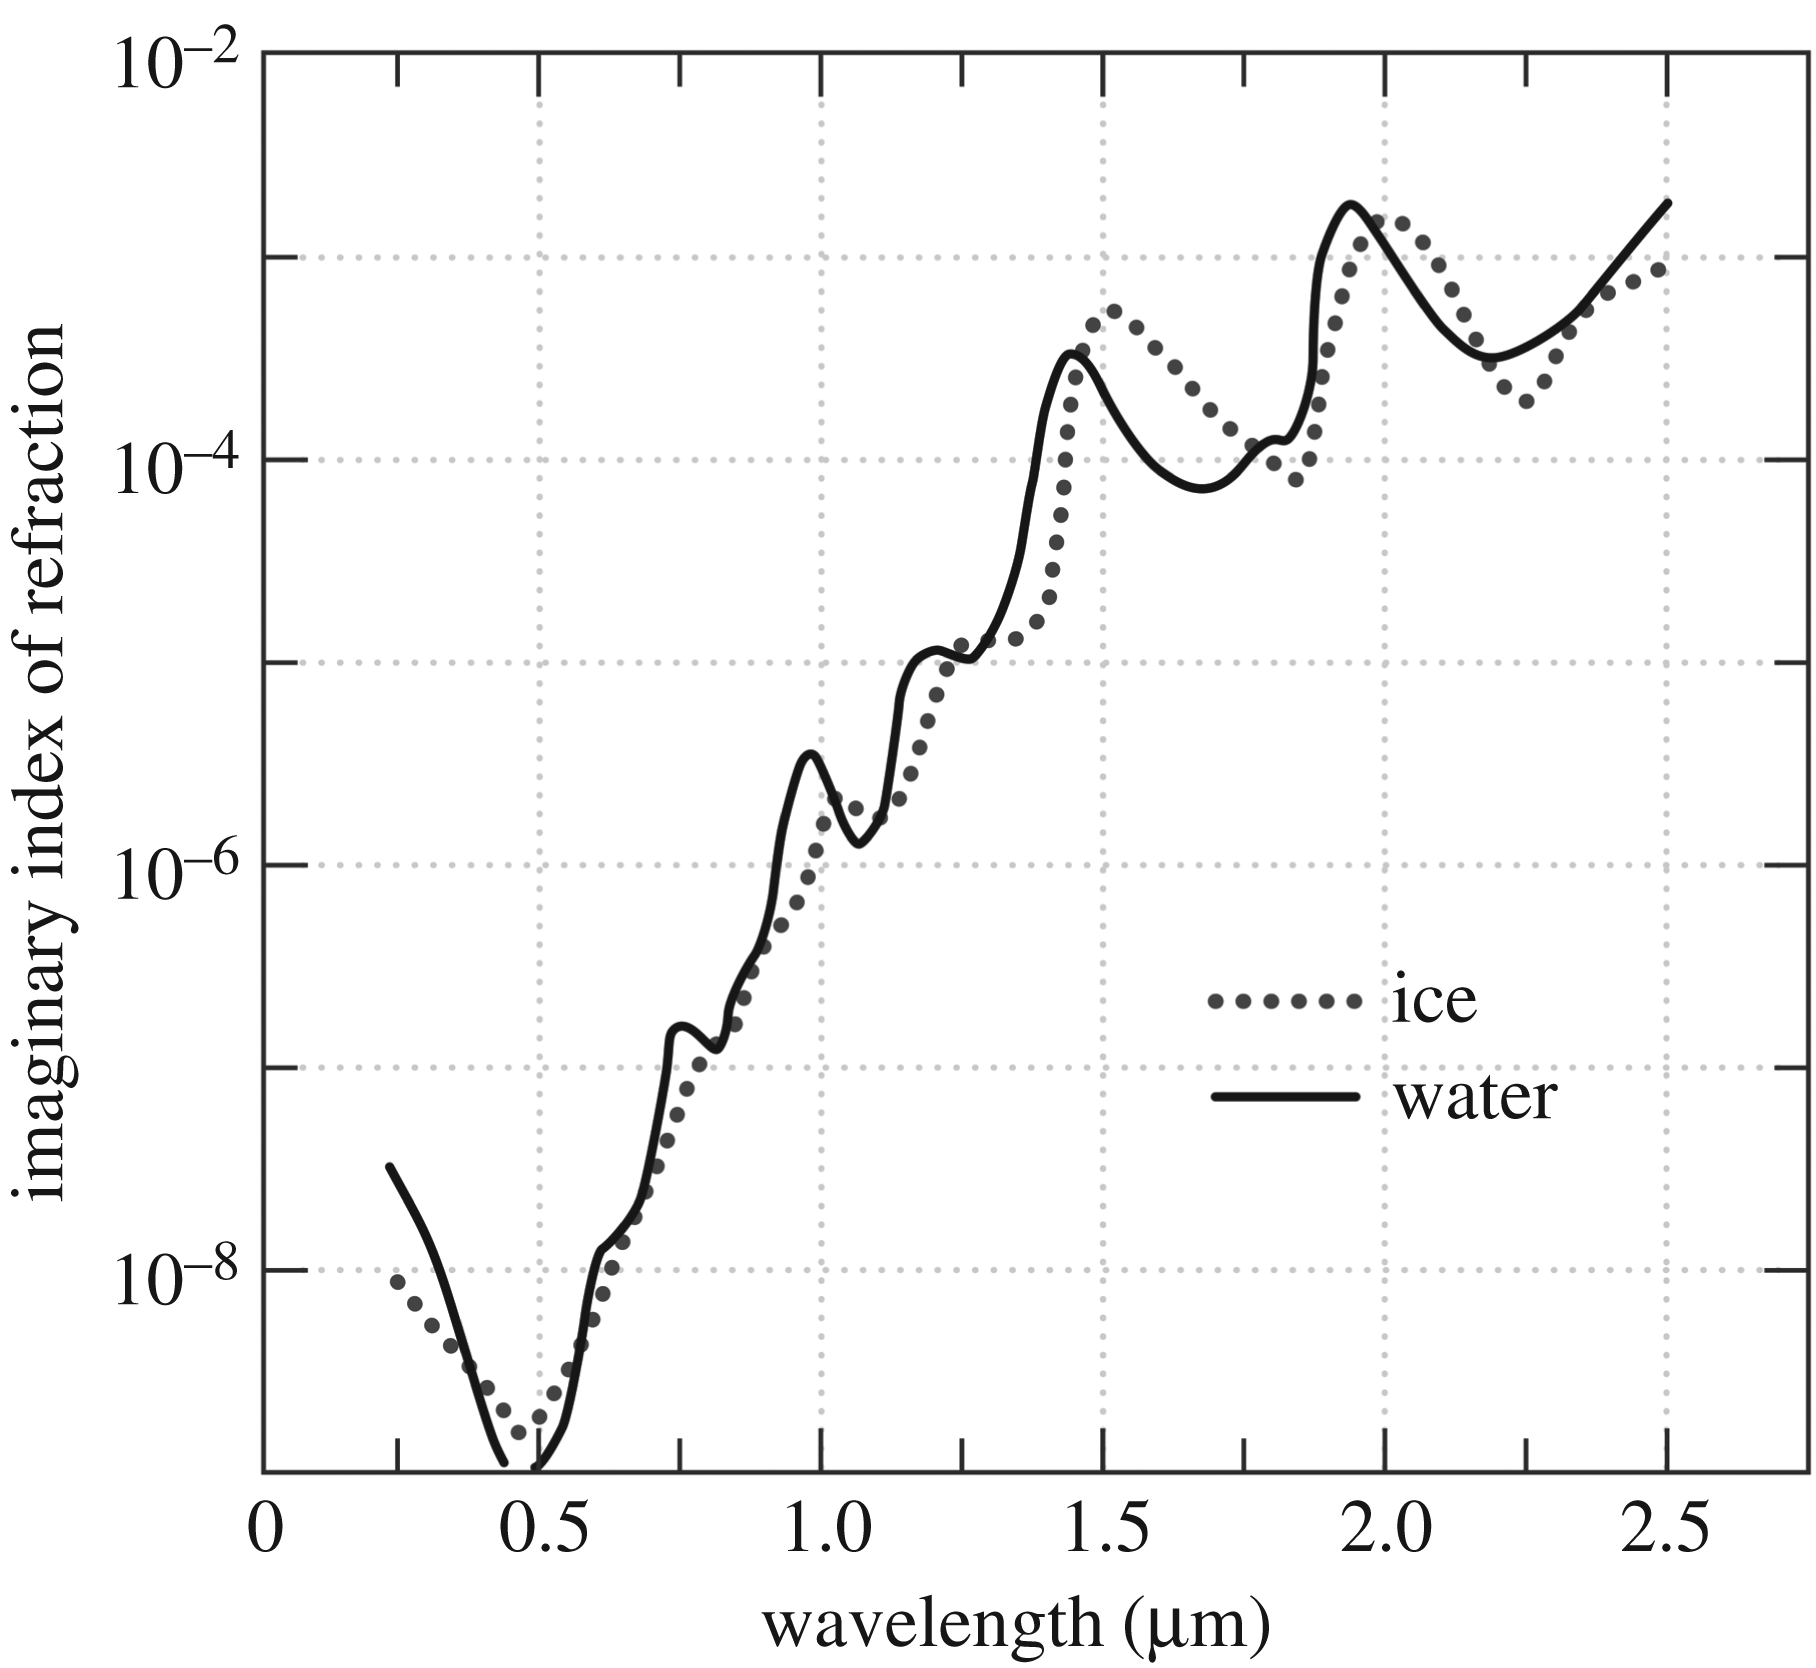
\includegraphics[width=0.5\textwidth]{figs/ch3/water_abs.png}
    \caption{\textbf{Water and Ice Absorption Spectra.}}{Absorption as the imaginary part of refraction (extinction coefficient), which is a measure of how much light is absorbed by a medium. The higher the extinction coefficient, the more light is absorbed by the medium. Taken from \textcite{dozierEstimationPropertiesAlpine1989}.}
    \label{fig:water}
\end{figure}
%----------------------------------------------------

Water is most transparent to radiation within the visible region (roughly 400 to 700 nm), outside this region radiation absorption increases rapidly. Near infrared radiation cannot penetrate far into water and is almost entirely absorbed. As seen in Figure \ref{fig:water}, water and ordinary hexagonal ice broadly have similar absorption characteristics across the visual and near infrared regions of the electromagnetic spectrum (\cite{warrenOpticalPropertiesIce2019}).

As the physical structure and composition of sea ice varies greatly, so do its optical properties. When seawater freezes and forms ice crystals, bubbles of gas and pockets of brine form between the crystals, leading to increased scattering across all wavelengths and thus a lower albedo. An increase in the thickness of ice leads to increased albedo, as seen in Figure \ref{fig:ice}. 

%----------------------------------------------------
\begin{figure}[H]
    \centering
    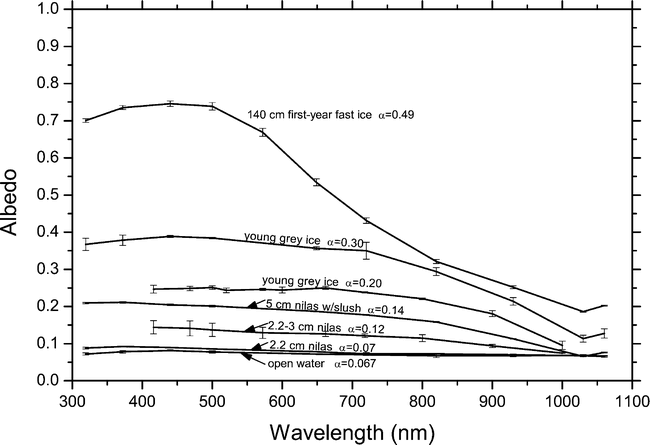
\includegraphics[width=0.65\textwidth]{figs/ch3/ice.png}
    \caption{\textbf{Various Ice Spectral Albedo.}}{Younger, less dense ice types such as first year ice have a higher albedo than older, denser ice types such as multi-year ice, this is due to the structure and composition of the different ice types. Taken from \textcite{brandtSurfaceAlbedoAntarctic2005}.}
    \label{fig:ice}
\end{figure}
%----------------------------------------------------

On average, snow has the highest albedo out of the three mediums, see Figure \ref{fig:snow}. The smaller the snow crystals, the higher the albedo. The denser the snow, the lower the albedo.

%----------------------------------------------------
\begin{figure}[H]
    \centering
    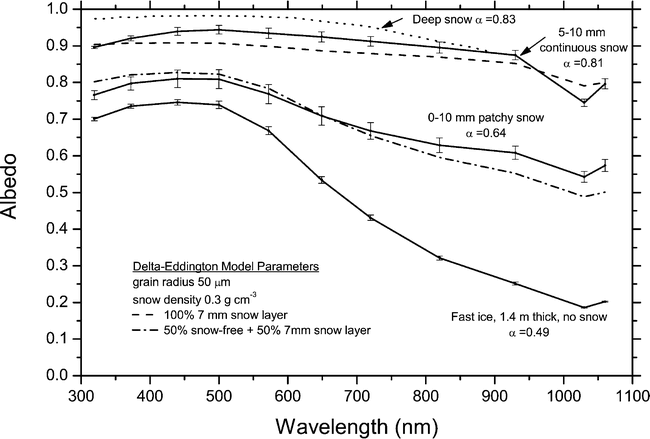
\includegraphics[width=0.65\textwidth]{figs/ch3/snow.png}
    \caption{\textbf{Snow Spectral Albedo.}}{Snow has a high albedo across the visual and near infrared regions of the electromagnetic spectrum, with the albedo increasing as the snow becomes less dense. Taken from \textcite{brandtSurfaceAlbedoAntarctic2005}.}
    \label{fig:snow}
\end{figure}
%----------------------------------------------------

The above suggests that the Livox Avia is best suited to detecting low density snow and first year ice, and it is unlikely to detect open water. Potentially, it may be possible for the sensor to detect ice floes of any ice type, given that they are likely to be covered with snow. It is likely that the return intensity values of points will vary significantly depending on the ice type and snow cover present  in the scene.

%====================================================
\section{Summary}
\label{sec:ch3:section6}
%----------------------------------------------------

\ac{LiDAR} sensors are becoming an increasingly popular method of remote sensing due to their ability to produce high-resolution 3D point clouds of their environment. Like any remote sensing method, \ac{LiDAR} has its unique advantages and disadvantages that must be considered when selecting a sensor for the desired application. The Livox Avia is a low-cost solid-state \ac{LiDAR} sensor with a unique non-repetitive scanning pattern that produces point clouds with a high number of points per frame with a non-uniform point distribution. Many common point cloud processing methods are built around the assumption that the input point cloud is in a standard grid format and that the target environment is likely to be an urban setting or one with simple geometries. These assumptions do not hold true for the data collected for this investigation, and will inform the methods selected for processing the collected point cloud data. The environmental features of interest in this investigation (sea ice and snow) has many complex interactions with electromagnetic radiation but is likely to reflect near-infrared radiation (the wavelength the Avia makes use of), while seawater is likely to absorb most of the emitted radiation. This suggests that the Avia is well suited for detecting sea ice and snow, but unlikely to detect open water.

%****************************************************
% END
%****************************************************